% use the aiaa-tc template.  TOTALLY SCREWED with it.
\documentclass[]{aiaa-tc}

% use the ACL bibliography format
\usepackage{acl_bibliography_style} 
 \title{Mining Interlinear Glossed Text Data for Determining Word Order in Resource-Poor Languages}

% write the title 
 \author{
  Thomas Marsh, \tt{tcmarsh@uw.edu}\\ University of Washington, CLMS, Ling 575, Winter Term, 2016, Fei Xia
 }

% Define commands to assure consistent treatment throughout document
\usepackage{xml}
\usepackage{tabularx} 
\usepackage{float}
\usepackage{parskip}

%%%%%%%%%%%%%%%%%%%%%%%%%%%%%%%%%%%%%%%%%%%%%%%%%%%%%%%%%%%%%%%%%%%%%%%%%%%%%%%%%%%%%%
\begin{document}

\maketitle

\begin{abstract}
This paper explores the process of using web-mined Interlinear-Glossed-Text (IGT) to determine typological features of resource-poor languages.  The typological features examined center around word order determination, however other features could be determined through a similar methodology.
\end{abstract}

\section*{Nomenclature}

\begin{tabbing}
  XXX \= \kill% this line sets tab stop
  $N$ \> Number of relevant IGT instances in individual languages \\
  $L_r$ \> Number of Languages which contain relevant IGT instances \\
  $L_e$ \> Number of Languages which were examined for a particular feature determination \\
  $L_t$ \> Total Number of languages \\
 \end{tabbing}

\section{Introduction}

Computational tools for examining typological properties of languages have become very powerful, however they tend to be focused around a small number of resource-rich languages such as English, Arabic, and Chinese.  In general, computational limitations of this nature are largely the result of two factors:   (1) Many computational algorithms require large amounts of data to function correctly.  This means that it is impossible, or very difficult to study resource-poor languages using these techniques.  (2) Existing computational tools, such as parsers, tend to have been trained on languages that have large amounts of labeled data available, and, as such, tend only to only exist for resource-rich languages.  Our approach to the first problem is to use web-mined IGT data as a corpus, \cite{lewis2006odin}.  For the second problem, we are using an English dependency parser \cite{de2006generating} to parse the IGT in translation, and then projecting this parse back across the gloss into the original language \cite{xia2007multilingual}.  Our contribution in the present work, is to apply these techniques to the problem of  determination of typological features for resource-poor languages, and discuss the accuracy of such determinations.  Specifically, the typological features we examine include word order for Subject, Object, Verb and Adjectives.  We validated this information using the World Atlas of Language Structures (WALS) \cite{wals}, \cite{haspelmath2005world}.

\section{Previous Work}

\subsection{Data Collection}
Collecting the ODIN data was done by the ODIN project in conjunction with LinguistList.  \cite{lewis2006odin}\\
Odin data was stored in XIGT format \cite{goodman2015xigt}\\
Enriching the ODIN data was done using the Stanford Parser \cite{xia2007multilingual} and \cite{de2006generating}\\

\subsection{Typological Feature Extraction with IGT Data}
cite Bender et al 2014 \cite{bender2014learning}\\
cite Bender et al 2013 \cite{goodman2013towards}\\
cite Lewis and Xia 2008 \cite{lewis2008automatically}\\

\section{Methodology}
% brief intro to methodology
Our general approach for these experiments was to read projected dependency parses from the enriched XIGT ODIN Data, and from them, determine the expected order of the parts of speech with respect to one another.  We do this for every language, and for every XIGT instance for which we have relevant data.  Whether or not we have relevant data is determined by whether there is an IGT instance which has been enriched with a projected dependency parse, and that dependency parse contains nodes which pass the heuristics for being relevant.  For each language, we then tally the determinations and divide each by the total to get the probability of the overriding orders.  If the order is below a certain threshold, then we set the value to NDO (No Discernable Order).

\begin{lstlisting}[language=python]
# loop through the languages
for language in languages:
    # loop through the igt for a language
    for igt in language:
        # if igt has projected dependency parse
        if igt.has_dependency_parse():
            dparse = igt.get_dependency_parse():
            # if the igt has the types for the specific words we are 
            # examining, e.g. if we are looking for adjective-noun order,
            # does this igt instance have a noun and an adjective with a head noun
            if dparse.has_usable_example():
                order = parse.get_order()
                # add one to the determined order count
                order_counts[order] += 1
                
\end{lstlisting}

\par
\subsection{Extracting and initial analysis}
In the XIGT format, the projected dependency-parse is indicated by the tier denoted "w-ds".  The dependency parse nodes are labeled with their stanford names (CITE!!).  The attribute \textit{dep} refers to the id of the word which is indicated by the labeled node.  The "w" tier indicates the words, and contains an offset into the original IGT lines, denoted \textit{segmentation}.  Segmentation is indicated by the line of text, and then a start, and end position in the target line.  We use these segmentations to compare the relative positions of the words.

For example, in the following XIGT data, we can see that the data says there is an adjective referring to a head noun.

\begin{lstlisting}[escapechar=@, language=XML, basicstyle=\sffamily, columns=fullflexible]
<igt id="igt430-14" `doc-id`="430" line-range="761-765" tag-types="L G+CR G+CR B T">
    <tier id="n" type="odin" alignment="c" state="normalized">
      <item id="n1" alignment="c1" line="761" tag="L">
        a. Ci         sono    @\bh@molti@\eh@ @\bh@clienti@\eh@ nel negozio.</item>
      <item id="n2" alignment="c2" line="762 763" tag="G+CR">
        EXPL        are     many clients in the store</item>
      <item id="n3" alignment="c3" line="764" tag="B" />
      <item id="n4" alignment="c4" line="765" tag="T">
        There are many clients in the store.</item>
    </tier>
    <tier id="p" type="phrases" content="n">
      <item id="p1" content="n1" />
    </tier>
    <tier id="w" type="words" segmentation="p">
      <item id="w1" segmentation="p1[0:2]" />
      <item id="w2" segmentation="p1[3:5]" />
      @\bh@<item id="w3" segmentation="p1[14:18]" />@\eh@
      @\bh@<item id="w4" segmentation="p1[22:27]" />@\eh@
      <item id="w5" segmentation="p1[28:35]" />
      <item id="w6" segmentation="p1[36:39]" />
      <item id="w7" segmentation="p1[40:48]" />
    </tier>
    <tier id="w-ds" type="dependencies" dep="w" head="w">
      <metadata type="intent-meta">
        <meta type="data-provenance" date="2016-01-11T15:29:18"
            method="projection" source="intent" />
      </metadata>
      <item id="w-ds1" dep="w2">root</item>
      <item id="w-ds2" dep="w1" head="w2" />
      @\bh@<item id="w-ds3" dep="w4" head="w2">nsubj</item>@\eh@
      @\bh@<item id="w-ds4" dep="w3" head="w4">amod</item>@\eh@
      <item id="w-ds5" dep="w7" head="w4">nmod:in</item>
      <item id="w-ds6" dep="w5" head="w7">case</item>
      <item id="w-ds7" dep="w6" head="w7">det</item>
    </tier>
/<igt>    
\end{lstlisting}

If we follow the highlighted sections up the tree and compare the locations of the adjective,\textit{w3} and the noun subject, \textit{w4} we can see that the adjective is referring to \textit{molti} and the noun is referring to \textit{clienti} and that, therefore, the adjective is preceding the noun in this instance.  Incidentally, according to the WALS gold standard data, this is incorrect for Italian; the noun should precede the adjective modifier.


\subsection{Heuristics for Word Order Determination}
The rules for determining word order were generally quite simple in order to get the purest results.

\subsubsection{Heuristics for SOV Order Determination}
\begin{itemize}
    \item Only Main Clause is examined.
    \item Passive sentences are not considered
    \item Dependency parse is considered if it has a \textit{dobj} and an \textit{nsubj} with head \textit{root}
    \item The Possible values are: "SOV", "SVO", "VSO", "VOS", "OVS", "OSV", and "NDO"
    \item NDO Threshold is set at 25%
\end{itemize}
\subsubsection{Heuristics for SV Order Determination}
\begin{itemize}
    \item Only Main Clause is examined.
    \item Passive sentences are not considered
    \item Dependency parse is considered if it has an \textit{nsubj} with head \textit{root}
    \item The Possible values are: "SV", "VS", and "NDO"
    \item NDO Threshold is set at 25%
\end{itemize}
\subsubsection{Heuristics for OV Order Determination}
\begin{itemize}
    \item Only Main Clause is examined.
    \item Passive sentences are not considered
    \item Dependency parse is considered if it has a \textit{dobj} with head \textit{root}
    \item The Possible values are: "OV", "VO", and "NDO" 
    \item NDO Threshold is set at 25%
\end{itemize}
\subsubsection{Heuristics for Adjective-Noun Determination}
\begin{itemize}
    \item Only Main Clause is examined.
    \item Dependency parse is considered if it has an \textit{amod} with head \textit{nn}, \textit{nsubj}, \textit{dobj}, or \textit{nsubjpass}
    \item The Possible values are: "Adjective-Noun", "Noun-Adjective", and "NDO"
    \item NDO Threshold is set at 25%
\end{itemize}
  
\subsection{Evaluation}
For evaluation, we compare our determinations to those from the World Atlas of Language Structure (WALS).  We do not consider languages for which WALS has no data.  We use the following chapters from WALS for our investigations.  

\begin{center}
Table 1: WALS Gold Standard
\end{center}
\begin{flushleft}
\begin{tabularx}{\textwidth}{|l|X|l|l|}
\hline
  \textbf{Word Orders Examined} & \textbf{Description} & \textbf{WALS Chapter} & \textbf{Citation} \\
\hline
SOV      & Order of Subject, Object, and Verb & 81A & \cite{wals-81}\\
\hline
SV       & Order of Subject and Verb          & 82A & \cite{wals-82}\\
\hline
OV       & Order of Object and Verb           & 83A & \cite{wals-83}\\
\hline
Adj-Noun & Order of Adjective and Noun        & 87A & \cite{wals-87}\\
\hline
\end{tabularx}
\end{flushleft}
\vspace{0.6cm}


\section{Results}
Experimental determination of word order using the projected dependency parses tended to match up relatively well with the gold standard data.  The amount of relevant IGT instances had a large impact on the accuracy of the data.  The best results were obtained by requiring at least 5 relevant IGT instances before counting and comparing the results.  This resulted in a relatively small number of languages which met the criteria for being usable.

%%%%%% INSERT GRAPH OF NUM LANGUAGES PER threshold
\begin{center}
Table 2: Experimental Results
\end{center}
\begin{flushleft}
\begin{tabularx}{\textwidth}{|l|X|l|l|}
\hline
  \textbf{Feature} & \textbf{Description} & \textbf{Accuracy} & \textbf{Num Languages Compared} \\
\hline
SOV      & Order of Subject, Object, and Verb & 79.01\% & 81\\
\hline
SV       & Order of Subject and Verb          & 85.14\% & 148\\
\hline
OV       & Order of Object and Verb           & 89.29\% & 112\\
\hline
Adj-Noun & Order of Adjective and Noun        & 75.00\% & 44\\
\hline
\end{tabularx}
\end{flushleft}
\vspace{0.6cm}


\section{Discussion and Error Analysis}

\subsection{Determining IGT Instances Threshold}
Predictably, we found that when the number of relevant IGT instances for a given language is low, the data tended to be somewhat unstable.  In order to quantify this, we examined several buckets of ranges of numbers of IGT instances, as well as several different cutoff thresholds.   Below, are four plots examining this data in two ways: (1) by setting a cutoff threshold of minimum acceptable number of instances for a language to be considered. (2) by setting several different "buckets" around ranges of numbers of instances of usable IGT.

\begin{figure}[H]
\caption{Number of Usable Languages per Range Buckets}
\hspace{-2mm} 
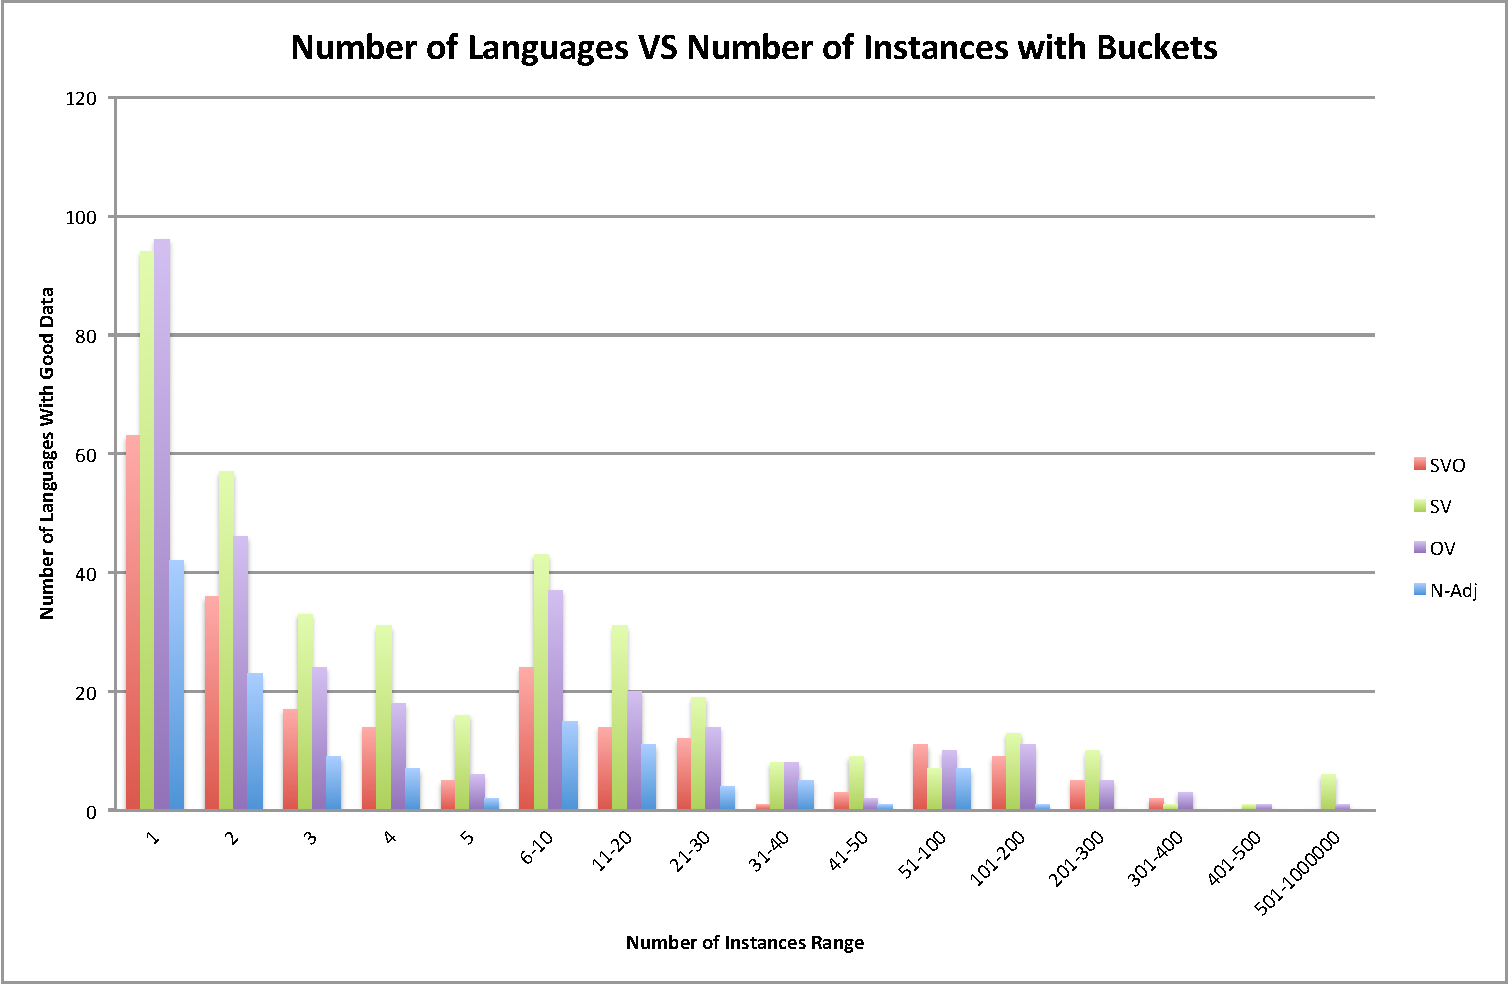
\includegraphics[width=\textwidth]{NumberOfLanguagesVsNumberOfInstancesWithBuckets.pdf}
\label{fig:label}
\end{figure}

\begin{figure}[H]
\caption{Accuracy per Range Buckets}
\hspace{-2mm} 
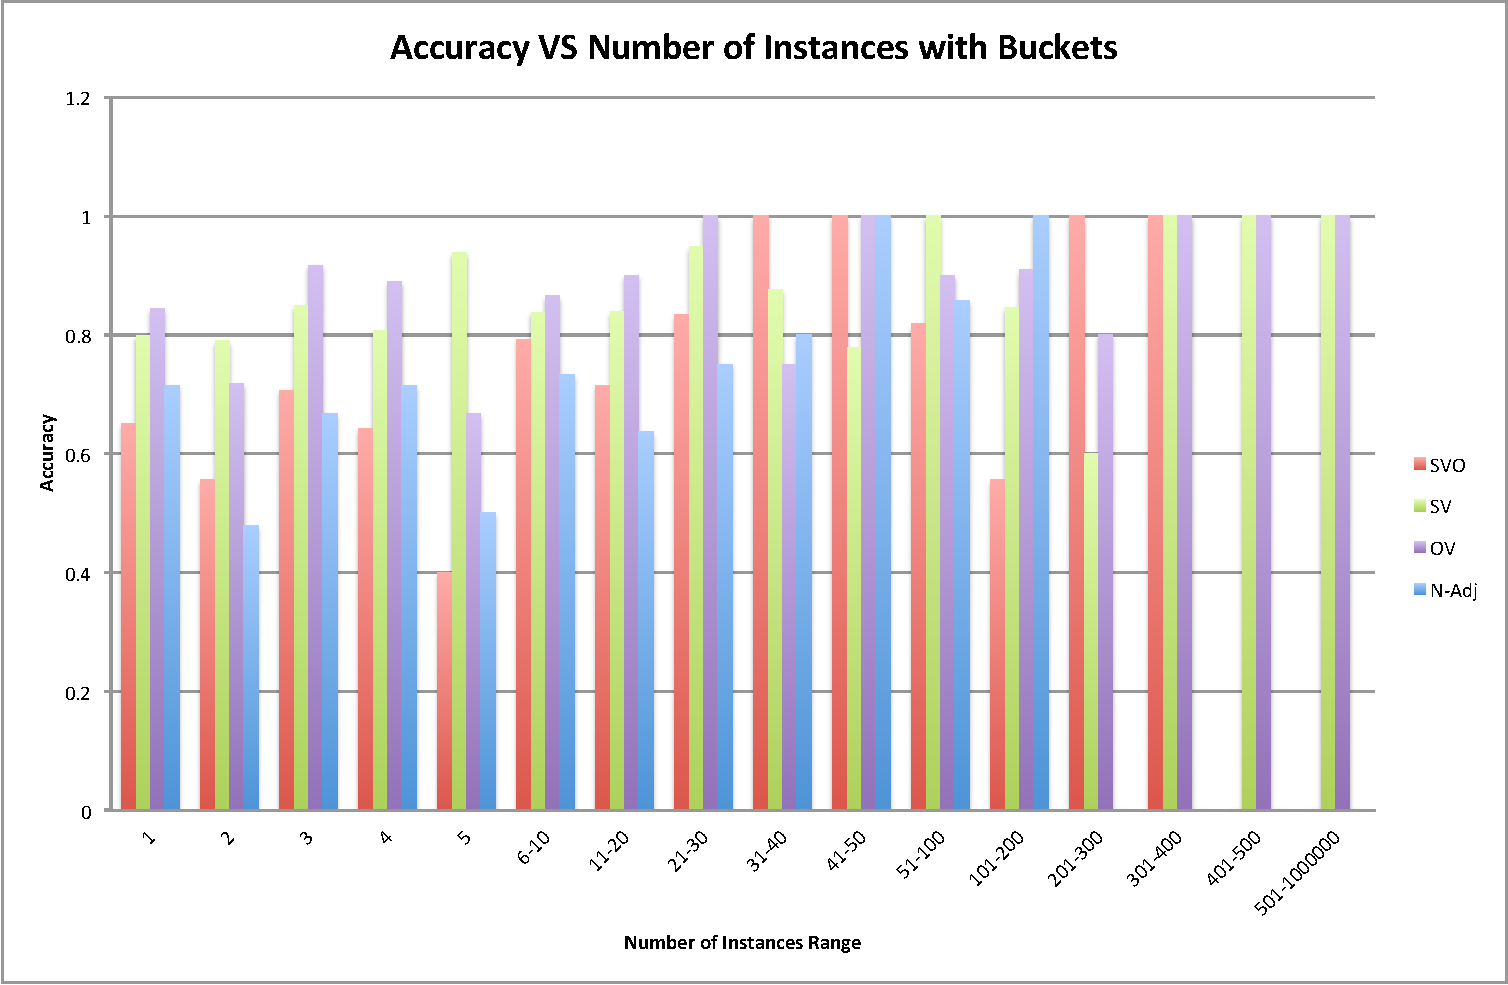
\includegraphics[width=\textwidth]{AccuracyVsNumberOfInstancesWithBuckets.pdf}
\label{fig:label}
\end{figure}

\begin{figure}[H]
\caption{Number of Usable Languages using Cutoff Threshold}
\hspace{-2mm} 
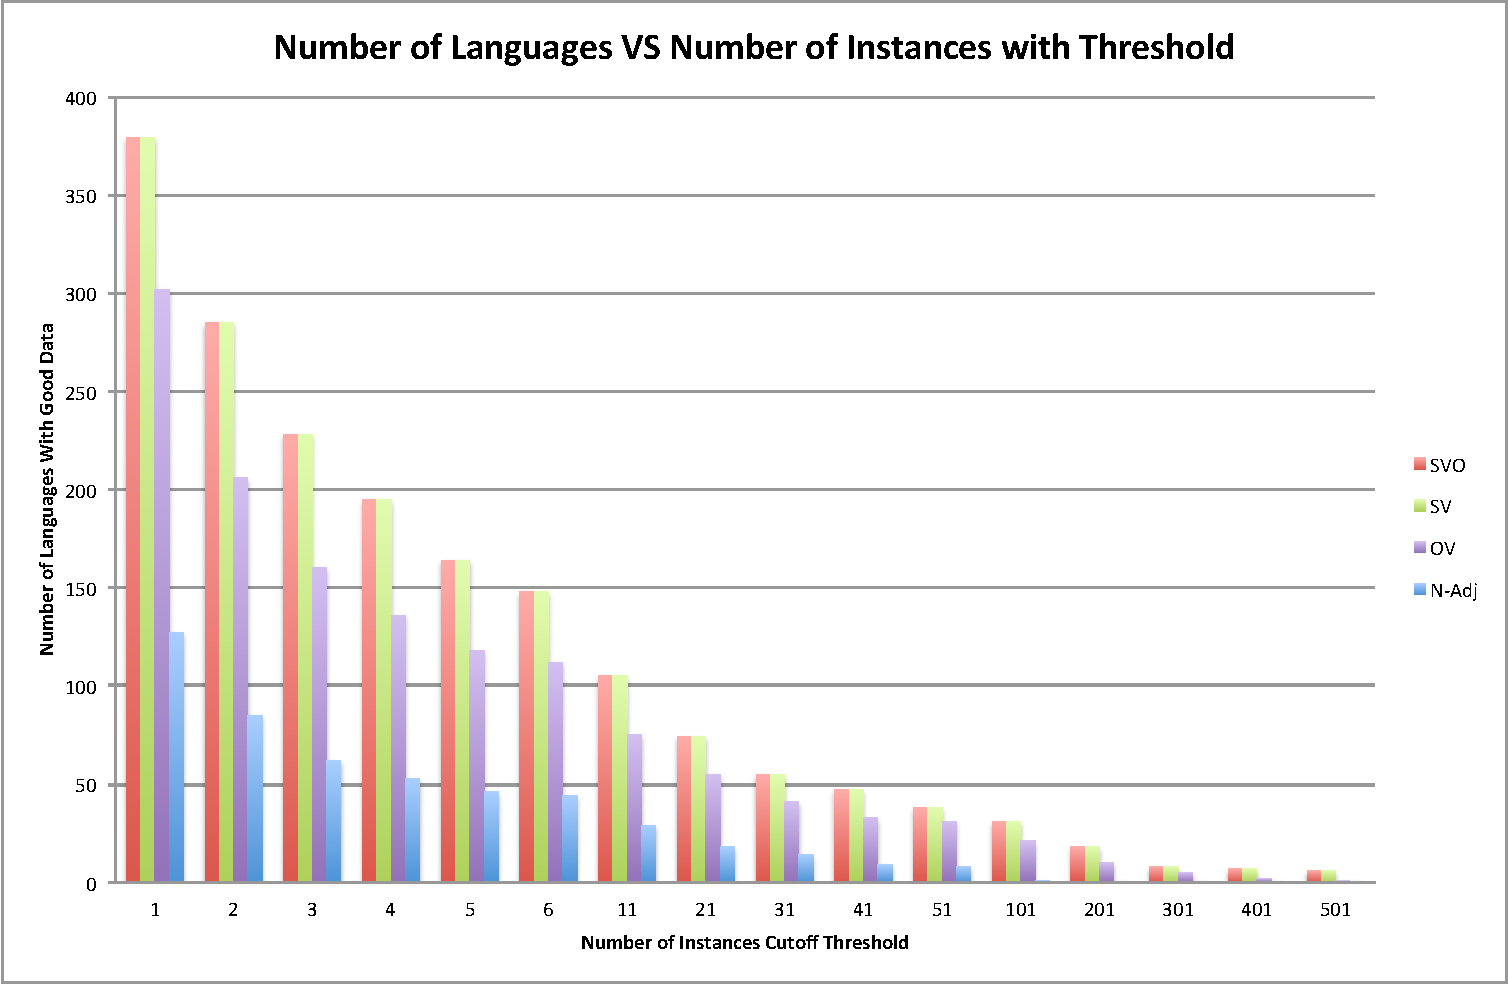
\includegraphics[width=\textwidth]{NumberOfLanguagesVsNumberOfInstancesWithThreshold.pdf}
\label{fig:label}
\end{figure}

\begin{figure}[H]
\caption{Accuracy when using Cutoff Threshold}
\hspace{-2mm} 
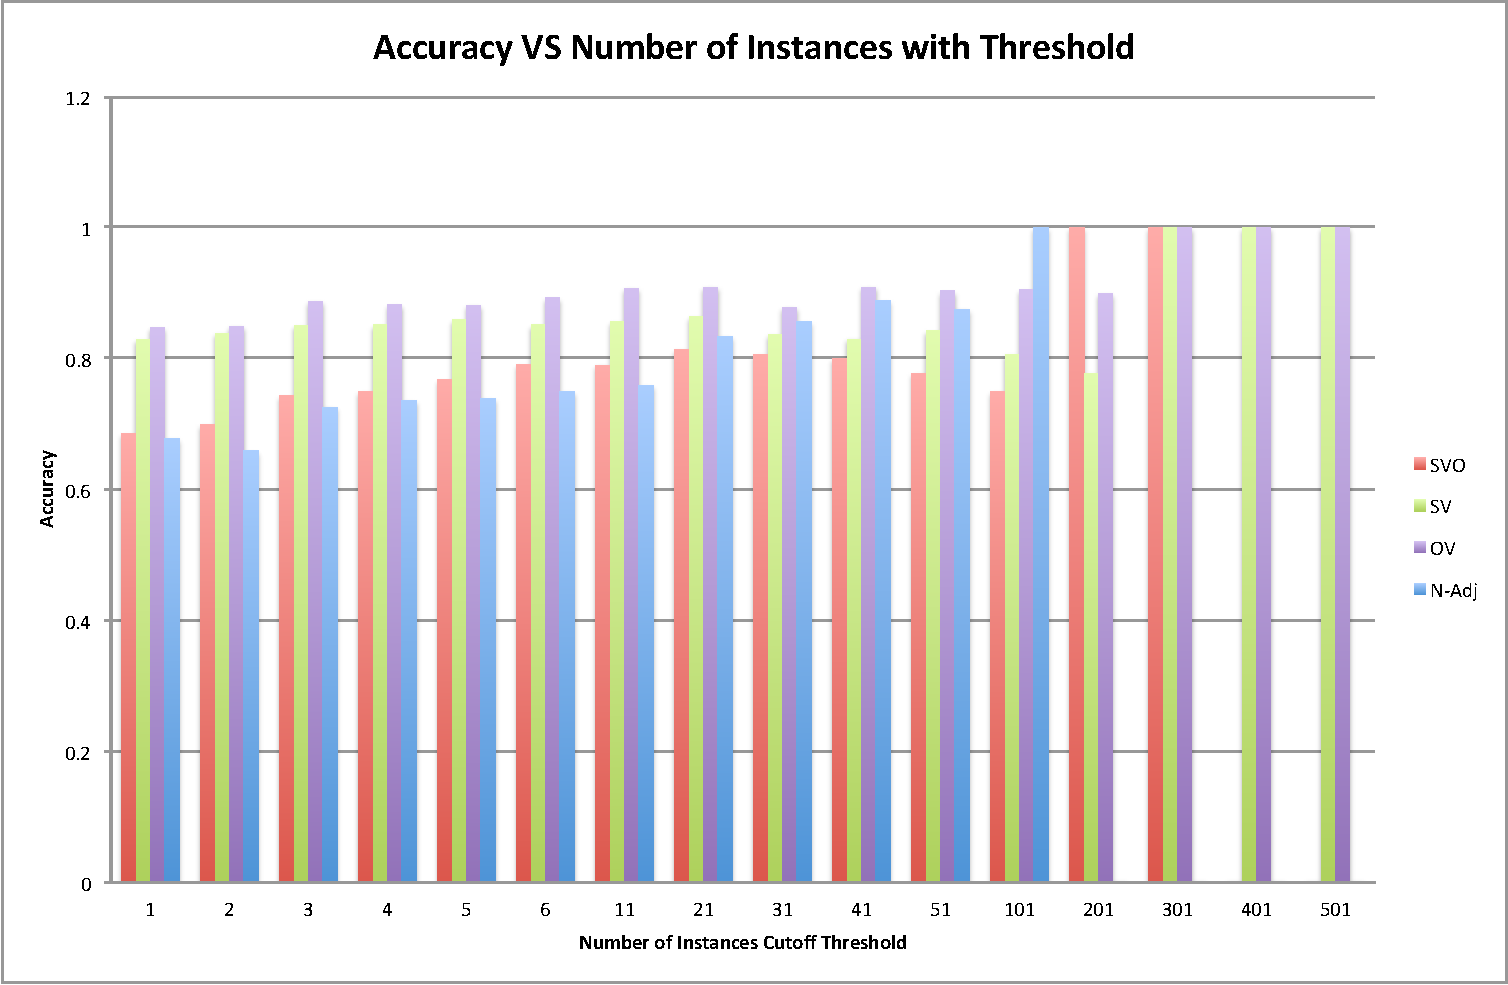
\includegraphics[width=\textwidth]{AccuracyVsNumberOfInstancesWithThreshold.pdf}
\label{fig:label}
\end{figure}

\subsection{NDO-Related Errors}
Though the results are encouraging, the lack of data and uncertainty around what the NDO threshold should be result in a fair amount of errors.  It can be observed in the following confusion matrices that the vast majority of incorrect assignments were NDO-Related.  These occur in both directions, i.e. when the gold standard determination is NDO, but our system's determination is something else, as well as when our system's determination is NDO and the gold standard determination is something else.  Note that in the confusion matrices, the row is the gold standard determination, and the column is the system determination.

\subsubsection{Subject Object Verb}
\begin{center}
Table 3: SOV Confusion Matrix
\end{center}
\begin{flushleft}
\begin{tabularx}{\textwidth}{|X|X|X|X|X|X|X|X|}
\hline
& \textbf{SOV} & \textbf{SVO} & \textbf{VSO} & \textbf{VOS} & \textbf{OVS} & \textbf{OSV} & \textbf{NDO} \\ \hline
\textbf{SOV} & 21  & 0   & 0   & 0   & 0   & 0   & 0  \\ \hline
\textbf{SVO} & 2   & 34  & 1   & 0   & 0   & 0   & 2  \\ \hline
\textbf{VSO} & 0   & 2   & 5   & 0   & 0   & 0   & 0  \\ \hline
\textbf{VOS} & 0   & 0   & 0   & 2   & 0   & 0   & 0  \\ \hline
\textbf{OVS} & 0   & 0   & 0   & 0   & 1   & 0   & 0  \\ \hline
\textbf{OSV} & 0   & 0   & 0   & 0   & 0   & 0   & 0  \\ \hline
\textbf{NDO} & 2   & 6   & 2   & 0   & 0   & 0   & 1  \\ \hline
\end{tabularx}
\end{flushleft}
\vspace{0.6cm}

\subsubsection{Subject Verb}
\begin{center}
Table 4: SV Confusion Matrix
\end{center}
\begin{flushleft}
\begin{tabularx}{\textwidth}{|X|X|X|X|}
\hline
& \textbf{SV} & \textbf{VS} & \textbf{NDO} \\ \hline
\textbf{SV} & 104  & 2   & 2   \\ \hline
\textbf{VS} & 5   & 22  & 0   \\ \hline
\textbf{NDO} & 12   & 1   & 0   \\ \hline
\hline
\end{tabularx}
\end{flushleft}
\vspace{0.6cm}

\subsubsection{Object Verb}
\begin{center}
Table 5: OV Confusion Matrix
\end{center}
\begin{flushleft}
\begin{tabularx}{\textwidth}{|X|X|X|X|}
\hline
& \textbf{OV} & \textbf{VO} & \textbf{NDO} \\ \hline
\textbf{OV} & 30  & 1   & 0   \\ \hline
\textbf{VO} & 4   & 70  & 1   \\ \hline
\textbf{NDO} & 4   & 2   & 0   \\ \hline
\hline
\end{tabularx}
\end{flushleft}
\vspace{0.6cm}

\subsubsection{Noun Adjective}
\begin{center}
Table 6: Noun-Adjective Confusion Matrix
\end{center}
\begin{flushleft}
\begin{tabularx}{\textwidth}{|X|X|X|X|}
\hline
& \textbf{Noun-Adjective} & \textbf{Adjective-Noun} & \textbf{NDO} \\ \hline
\textbf{Noun-Adjective} & 12  & 3   & 4   \\ \hline
\textbf{Adjective-Noun} & 1   & 21  & 2   \\ \hline
\textbf{NDO} & 0   & 1   & 0   \\ \hline
\hline
\end{tabularx}
\end{flushleft}
\vspace{0.6cm}


\section{Conclusion}


\pagebreak

\bibliographystyle{acl}
\bibliography{references}

\end{document}


